\documentclass[main.tex]{subfiles}

\begin{document}
\section{Implementation}\label{sec:implementation}

\subsection{Frontend webapp implementation}
The frontend of this app has been developed using Flutter, written in the Dart programming language, then compiled to run on the web.
Flutter is a multi-platform framework to make apps, both on mobile and desktop, including the web, as in this case.

The software architecture of this app follows a Single Page Application pattern, where the webapp is rendered in the browser. Moreover, in this specific case, no HTML or CSS is used. But instead the content is rendered on a web canvas using CanvasKit.

Finally, its interoperability with JavaScript allowed the use of Web3.js APIs as usual.

It is \textbf{currently hosted via GitHub Pages} on \href{https://gethdomains.best}{https://gethdomains.best}, compiled using a CI/CD pipeline on GitHub Actions at every push on the repository.

\subsubsection{Data flow across software layers}
The flow of data when communicating with the Smart Contract is interesting and more focused on design patterns such as BLoC (summarized in figure \ref{fig:dart_invocations_dataflow}):
\begin{itemize}
    \item the user interface is made up of Widgets, the core element for the UI
    \item in most of the cases, when a user input is required, the text field is attached to a Reactive Form, with real-time client-side validations to provide a better UX when the user inputs data that is not in the right format
    \item input data is then collected in a model object, to be sent to the business logic of the application, implemented using BLoCs
    \item inside of a BLoC is kept the state of the application, such as the current balance, the list of domains currently for sale, and so on; that allows various parts of the webapp to interact with the global state in a reactive and decoupled way
    \item then data has a first transformation, from a model or an event to simpler data structures to be sent to the Repository layer which is at a lower abstraction level with respect to the actual Smart Contract interaction code
    \item the Repository will transform data such as domain names from String to the data type that the Smart Contract requires in input, such as byte arrays (in Dart: Uint8List)
    \item the invocation is now at the level of the smart contract Dart class: this is responsible for the call of the JavaScript code from Dart; for instance, byte arrays and more complex data types must be simplified in order to be serialized then sent to a function written in a completely different language such as JavaScript (Uint8List may become base64 strings, structs may be sent or received as JSON strings, and so on)
    \item finally, the call has reached the JavaScript code, where the web3.js API stands and can be used to make the actual feature requested: whatever we had before is just an abstraction layer required to drastically improve the quality of the code thanks to the decoupling of responsibilities, according to the SRP principle
\end{itemize}

\begin{figure}[htbp]
    \centering
    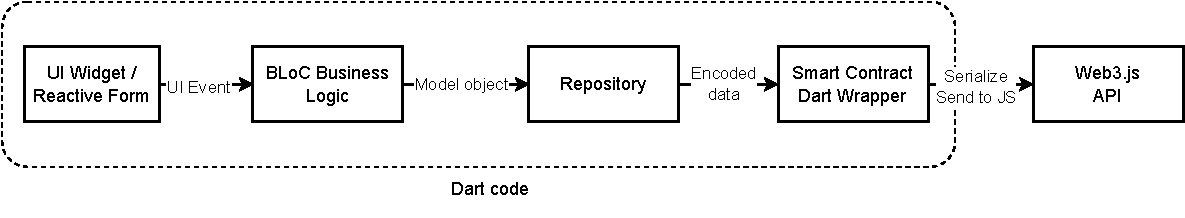
\includegraphics[width=\textwidth]{figures/dart_invocations_dataflow.pdf}
    \caption{Layered architecture overview}
    \label{fig:dart_invocations_dataflow}
\end{figure}

\subsubsection{Transaction hash immediately available}
As soon as the transaction is sent, a transaction hash is available and it's good practice to inform the user of this result.
To do that, on the JavaScript side the asynchronous function call is handled using Promises, which will be translated on the Dart side as Futures, but the conceptual meaning is exactly the same.
At this point, a global event of this transaction is propagated and the user sees a nice looking banner, with a link to Etherscan to actually see his transaction. Also, the global state cannot be updated so soon, because the transaction is not mined in a confirmed block yet.

After some time, the transaction will be confirmed and the events emitted will also be received.
Only here and now we are able to update the global state informing the user of the success of the action. Updating the global state (contained in a BLoC) will trigger a reactive redraw of elements of the UI affected by the change.

\subsubsection{Fees estimation}
Right before sending a transaction, a local pre-check is made. The gas fees are estimated calling the corresponding API provided by web3.js (which leverages on the Etherum provider, often Metamask).
The noticeable here is that, in case the smart contract will raise an error and revert its execution given the current local state of the Smart Contract, the user will be notified immediately, without the need to send a transaction that will likely fail.

Moreover, the gas fees estimation is useful and displayed interactively to the user when its input is able to affect the fees required, in order to make it more aware.

\subsubsection{Login management}
The login procedure, when connected to Metamask or another compatible provider, is basically the request of the permission to read a registered Ethereum account.
In case the app can do that right away, the permission was already granted and the user can be considered logged in.

Different story regarding the logout: it is implemented artificially by saving that in the state of the app and making it persistent across refreshes of the page (i.e.: localStorage in the browser, but abstracted using HydratedBLoC).

\subsubsection{Settings}
A few settings are available for the user to change:
\begin{itemize}
    \item the IPFS gateway is one of the most important ones because supposing the anti-censorship goal of the service, in case one provider gets blocked or simply it is down for a while, another one can be freely chosen and used
    \item to improve the UX of the app, a setting on Dark and Light theme is made: the default setting is to follow the brightness of the operating system and therefore the current browser
\end{itemize}

\subsubsection{Metamask integration}
Metamask is considered key in the UX improvement.

After the user buys our token for the first time, a Metamask prompt will pop-up (figure \ref{fig:metamask_notification_prompts}) asking to add the ERC-20 token to the wallet directly, via the \texttt{wallet\_watchAsset} API. It allows the user to have an eye on his balance right from Metamask, but also send and receive tokens directly by interacting with the wallet.
Since the smart contract implements the ERC-20 interface and the frontend webapp handles the Transfer events, this approach is totally fine and incentivized by showing the Metamask dialog.

A very similar approach is used for the domain, which is actually an NFT. Its contract implements the ERC-721 interface and the webapp allows the user to add the domain in the Metamask NFT subsection, allowing traditional token exchange outside of the webapp. As before, the webapp handles this situation just fine and in a reactive way listening to the Transfer events emitted by the smart contract.

\begin{figure}[htbp]
    \centering

    \begin{subfigure}[t]{0.45\textwidth}
        \centering
        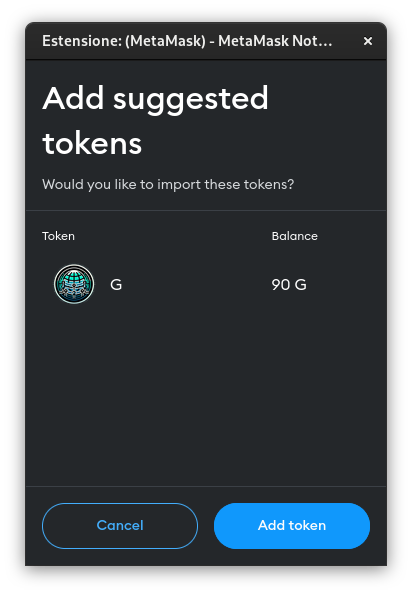
\includegraphics[width=\textwidth]{figures/metamask_prompt_add_geth_token_erc20.png}
        \caption{Prompt for ERC-20 token}
    \end{subfigure}
    \begin{subfigure}[t]{0.45\textwidth}
        \centering
        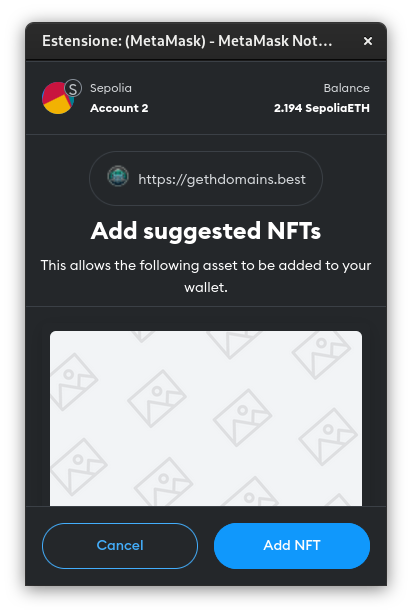
\includegraphics[width=\textwidth]{figures/metamask_prompt_add_geth_domain_nft.png}
        \caption{Prompt for ERC-721 token}
    \end{subfigure}
    
    \caption{Metamask dialogs}
    \label{fig:metamask_notification_prompts}
\end{figure}

\subsubsection{Encoder library}
The logic to encode and decode multiple types of data is considered distinct from the app itself from a code recycle perspective, so it was worth making it a totally separate library.

It has the advantage of being reusable and cross-compilable, from desktop apps (on Windows, OS X, Linux) to mobile apps (Android, iOS) but also on the web (both JavaScript or WebAssembly) thanks to the power of the Dart programming language.

In our specific situation, it was also compiled as a CLI app that runs on Linux, for testing purposes when the webapp didn't exist yet (as can be seen in figure \ref{fig:data_encoder_cli_usage}).

\begin{figure}[htbp]
    \centering
    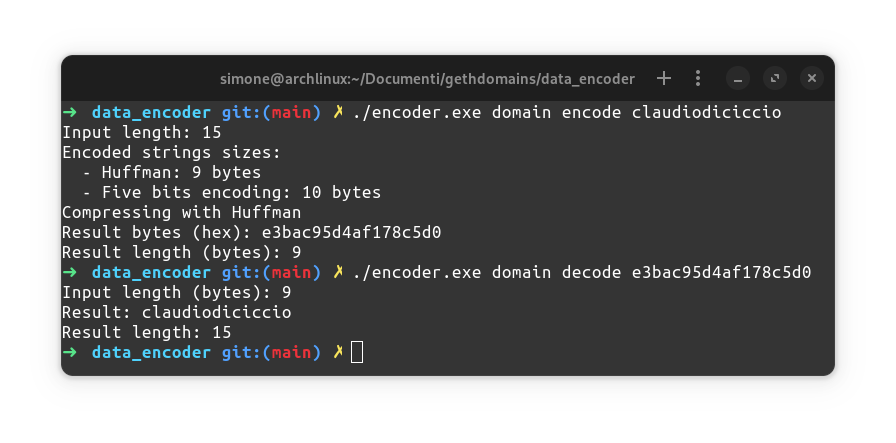
\includegraphics[width=0.85\textwidth]{figures/data_encoder_cli_usage}
    \caption{Example usage of the encoder library via CLI}
    \label{fig:data_encoder_cli_usage}
\end{figure}

The library offers the logic to encode and decode various data:
\begin{itemize}
    \item domain names, using a mixed encoding strategy (Huffman trees or using 5 bits to encode each character)
    \item Tor Onion v3 addresses, extracting the ECDSA public key
    \item IPFS CID, extracting only the multihash and multicoded parts of the specification
\end{itemize}

It also provided a command line interface, with a short help page, to make it usable in a simple way.

\subsubsection{Future progress for the webapp}
As we had the possibility to observe the webapp layered architecture in one of the previous subsections, it's obvious as the only layer in which the actual platform native implementation shows up is right before calling the JavaScript function. All the business logic and the high level transformations are totally separated and recyclable.

In practical terms, this means that it would be relatively easy to just reimplement the calls to the smart contract using another library (for example a wrapper that calls the Metamask mobile app), then the webapp will immediately be compilable for another operating system, making it an Android or iOS app in little time, just as an example.

\subsubsection{Screenshots}
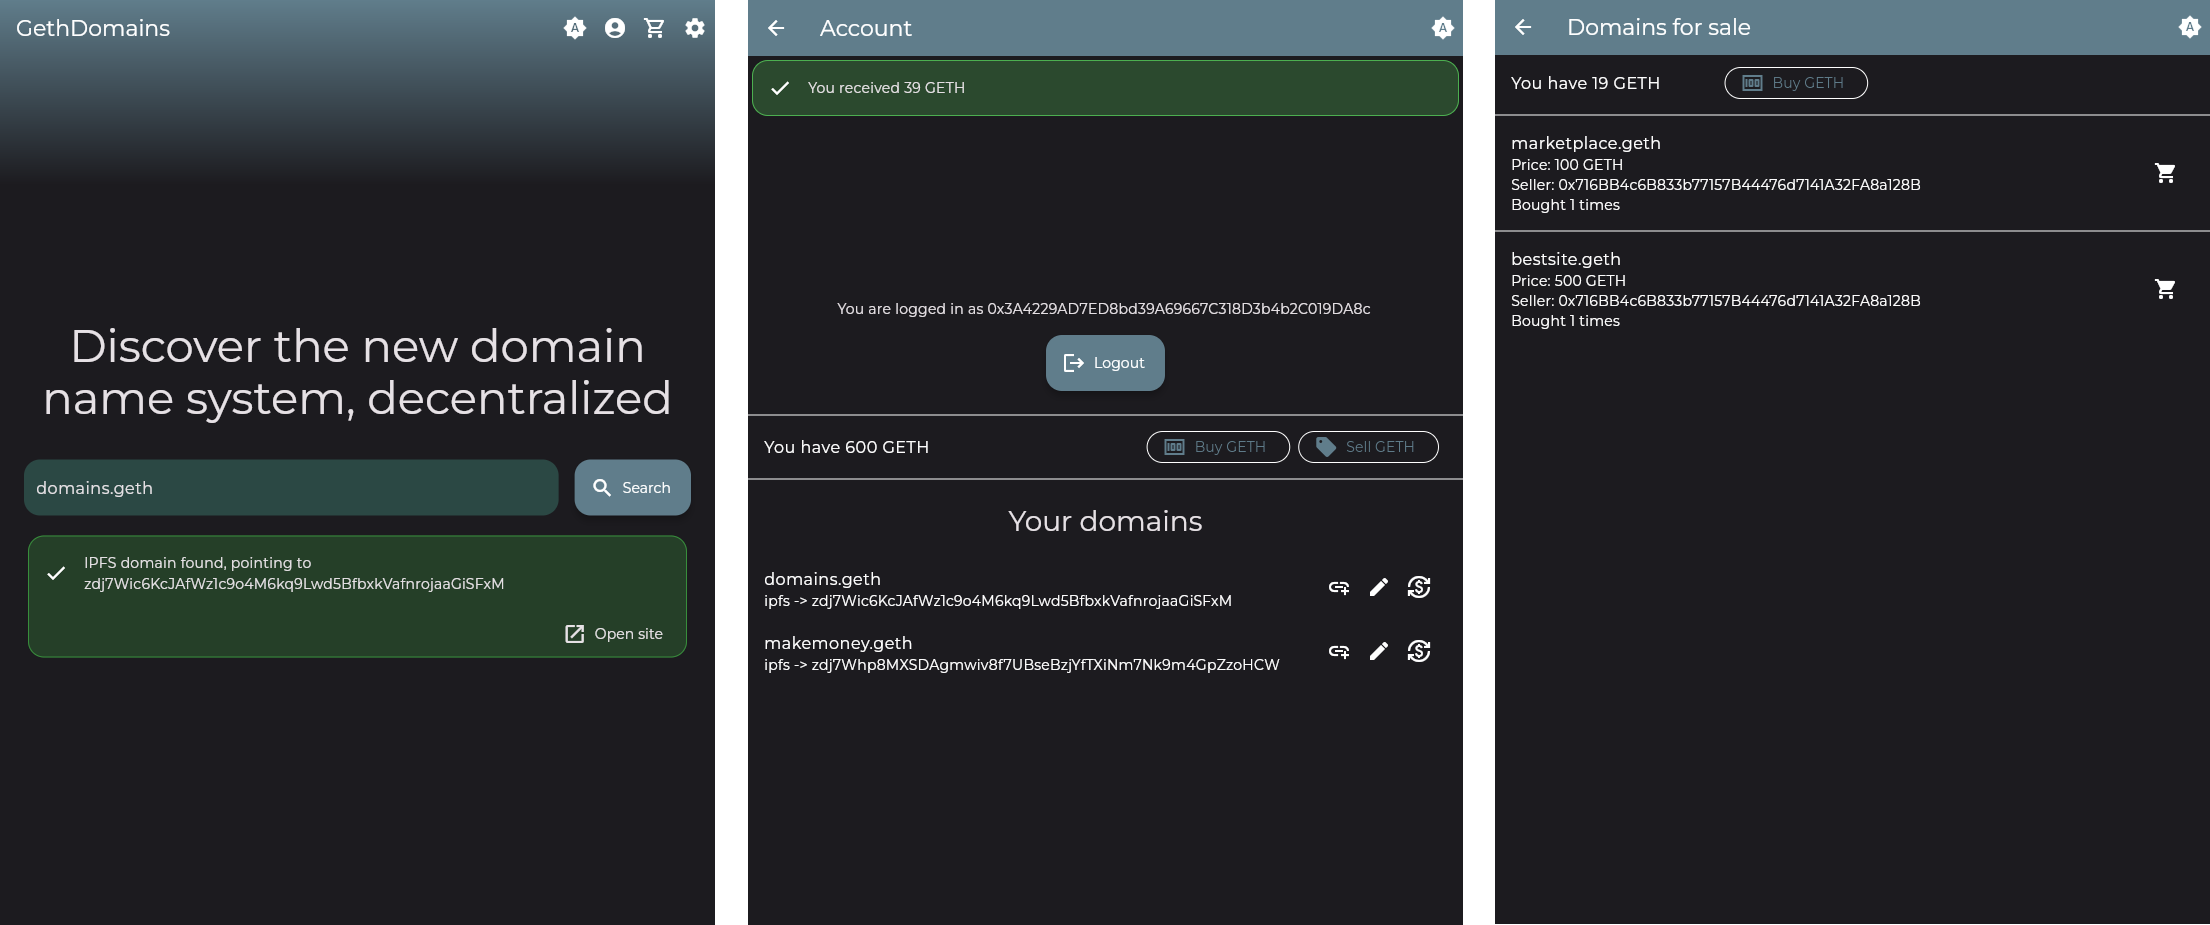
\includegraphics[width=\textwidth]{figures/webapp_screenshot_carousel.png}

\subsection{Smart Contracts}

\subsubsection{OpenZeppelin library}
To minimize the risk of vulnerabilities we used the \texttt{OpenZeppelin} library which provides heavily tested contracts that implement the interfaces defined by the ERC standards. To represent a domain, a non-fungible token, we implemented the ERC721Royaltee's interface in our smart contract DomainMarketplace. Its interface allows us to represent NFTs and manage their transfer and the possible amount of royalties that the creator of a domain would expect. For the  Geth token, used for the purchase of a domain, we extended the erc20 contract of OpenZeppelin which is used to represent fungible tokens.

\subsubsection{Tools adopted}
The testing of the smart contracts was made using 2 different environments.

The first one is composed by \texttt{Truffle} and \texttt{Ganache}. Truffle was used to deploy smart contracts and work on them through the truffle console. To optimize the testing we wrote some JavaScript tests. Ganache was used as a workspace where the changes to the state of the blockchain were visible.
The JavaScript tests were made on the main functionalities of the smart contracts:
\begin{itemize}
    \item For the GethDomain.sol the functions called to buy a new domain or an existing domain were tested, checking if the state of the contract and the user account were consistent with the amount of Geth spent, and that the data was stored correctly in the chain. Tests were made on the functions to sell and retrieve an owned domain too, checking the data consistency and the specified constraints on the permissions of these.
    \item For Geth.sol the test consists of purchasing and selling the token, checking the consistency of the balances.
\end{itemize}

The second one was made through the deployment on \texttt{Sepolia} and using \texttt{remix} with \texttt{metamask} to interface with the testenet.
Testnets\cite{Sepolia} are blockchains designed to mimic the operating environment of a mainnet but exist on a separate ledger.  Sepolia ETH is the currency used to pay to complete transactions on the Sepolia testnet, similar to how ETH is used to pay for computation on Ethereum’s mainnet.


\end{document}